\documentclass[12pt,oneside]{paper}

\usepackage{listings}
\renewcommand{\lstlistingname}{saucecode}

\lstset{%
  language={C},
  basicstyle={\small},%
  identifierstyle={\small},%
  commentstyle={\small\itshape},%
  keywordstyle={\small\bfseries},%
  ndkeywordstyle={\small},%
  stringstyle={\small\ttfamily},
  frame={tb},
  breaklines=true,
  columns=[l]{fullflexible},%
  numbers=left,%
  xrightmargin=0zw,%
  xleftmargin=3zw,%
  numberstyle={\scriptsize},%
  stepnumber=1,
  numbersep=1zw,%
  lineskip=-0.5ex%
}



% タイトル
\title{マルチコプターの高度制御についての研究}
\author{又村 峰裕}

\begin{document}
% 行間
\setlength{\baselineskip}{9truemm}

%文字間
\kanjiskip=.53zw plus 3pt minus 3pt
\xkanjiskip=.53zw plus 3pt minus 3pt

% 目次
\tableofcontents
%\newpage

% 本文
\chapter{はじめに}

\section{研究の背景}
ドローンとは,無人で遠隔操作や自動制御によって飛行できる航空機の総称のことである.ドローンの始まりは図1.1に示す軍事用に偵察や攻撃用に作られたプレデターが始まりである.近年,図1.2に示す宅配サービスや図1.3に示す農薬を撒く農業用,図1.4図1.5に示す空撮,水中撮影,図1.6に示す掌に収まるくらいの小型用,図1.7に示す娯楽等のドローンが普及してきた.3つ以上のメインローターを持つヘリコプターをマルチコプターと呼び,その中から4つのメインローターを持つクアッドコプター図1.8について研究する.室内で使うことのできるマルチコプターは多くない.

\begin{figure}[htbp]
  \begin{center}
    \includegraphics[width=100mm]{img/図1.jpg}
    \end{center}
  \caption{プレデタ―}
 \label{fig:robot}
\end{figure}

\begin{figure}[htbp]
  \begin{center}
    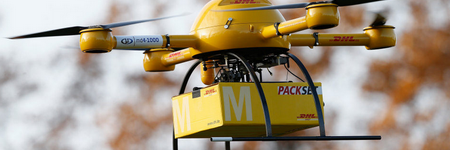
\includegraphics[width=100mm]{img/ドローンの商業利用.png}
    \end{center}
  \caption{商業用}
 \label{fig:robot}
\end{figure}

\begin{figure}[htbp]
  \begin{center}
    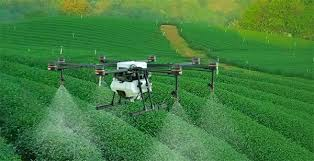
\includegraphics[width=100mm]{img/images.jpg}
    \end{center}
  \caption{農業用}
 \label{fig:robot}
\end{figure}

\begin{figure}[htbp]
  \begin{center}
    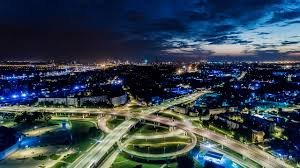
\includegraphics[width=100mm]{img/空撮.jpg}
    \end{center}
  \caption{空撮}
 \label{fig:robot}
\end{figure}

\begin{figure}[htbp]
  \begin{center}
    \includegraphics[width=100mm]{img/図2.jpg}
    \end{center}
  \caption{水中撮影用}
 \label{fig:robot}
\end{figure}

\begin{figure}[htbp]
  \begin{center}
    \includegraphics[width=100mm]{img/図3.jpg}
    \end{center}
  \caption{小型の娯楽用}
 \label{fig:robot}
\end{figure}

\begin{figure}[htbp]
  \begin{center}
    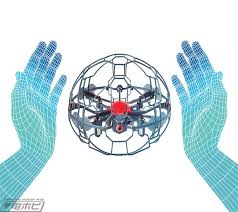
\includegraphics[width=100mm]{img/ダウンロード.jpg}
    \end{center}
  \caption{娯楽用}
 \label{fig:robot}
\end{figure}

\begin{figure}[htbp]
  \begin{center}
    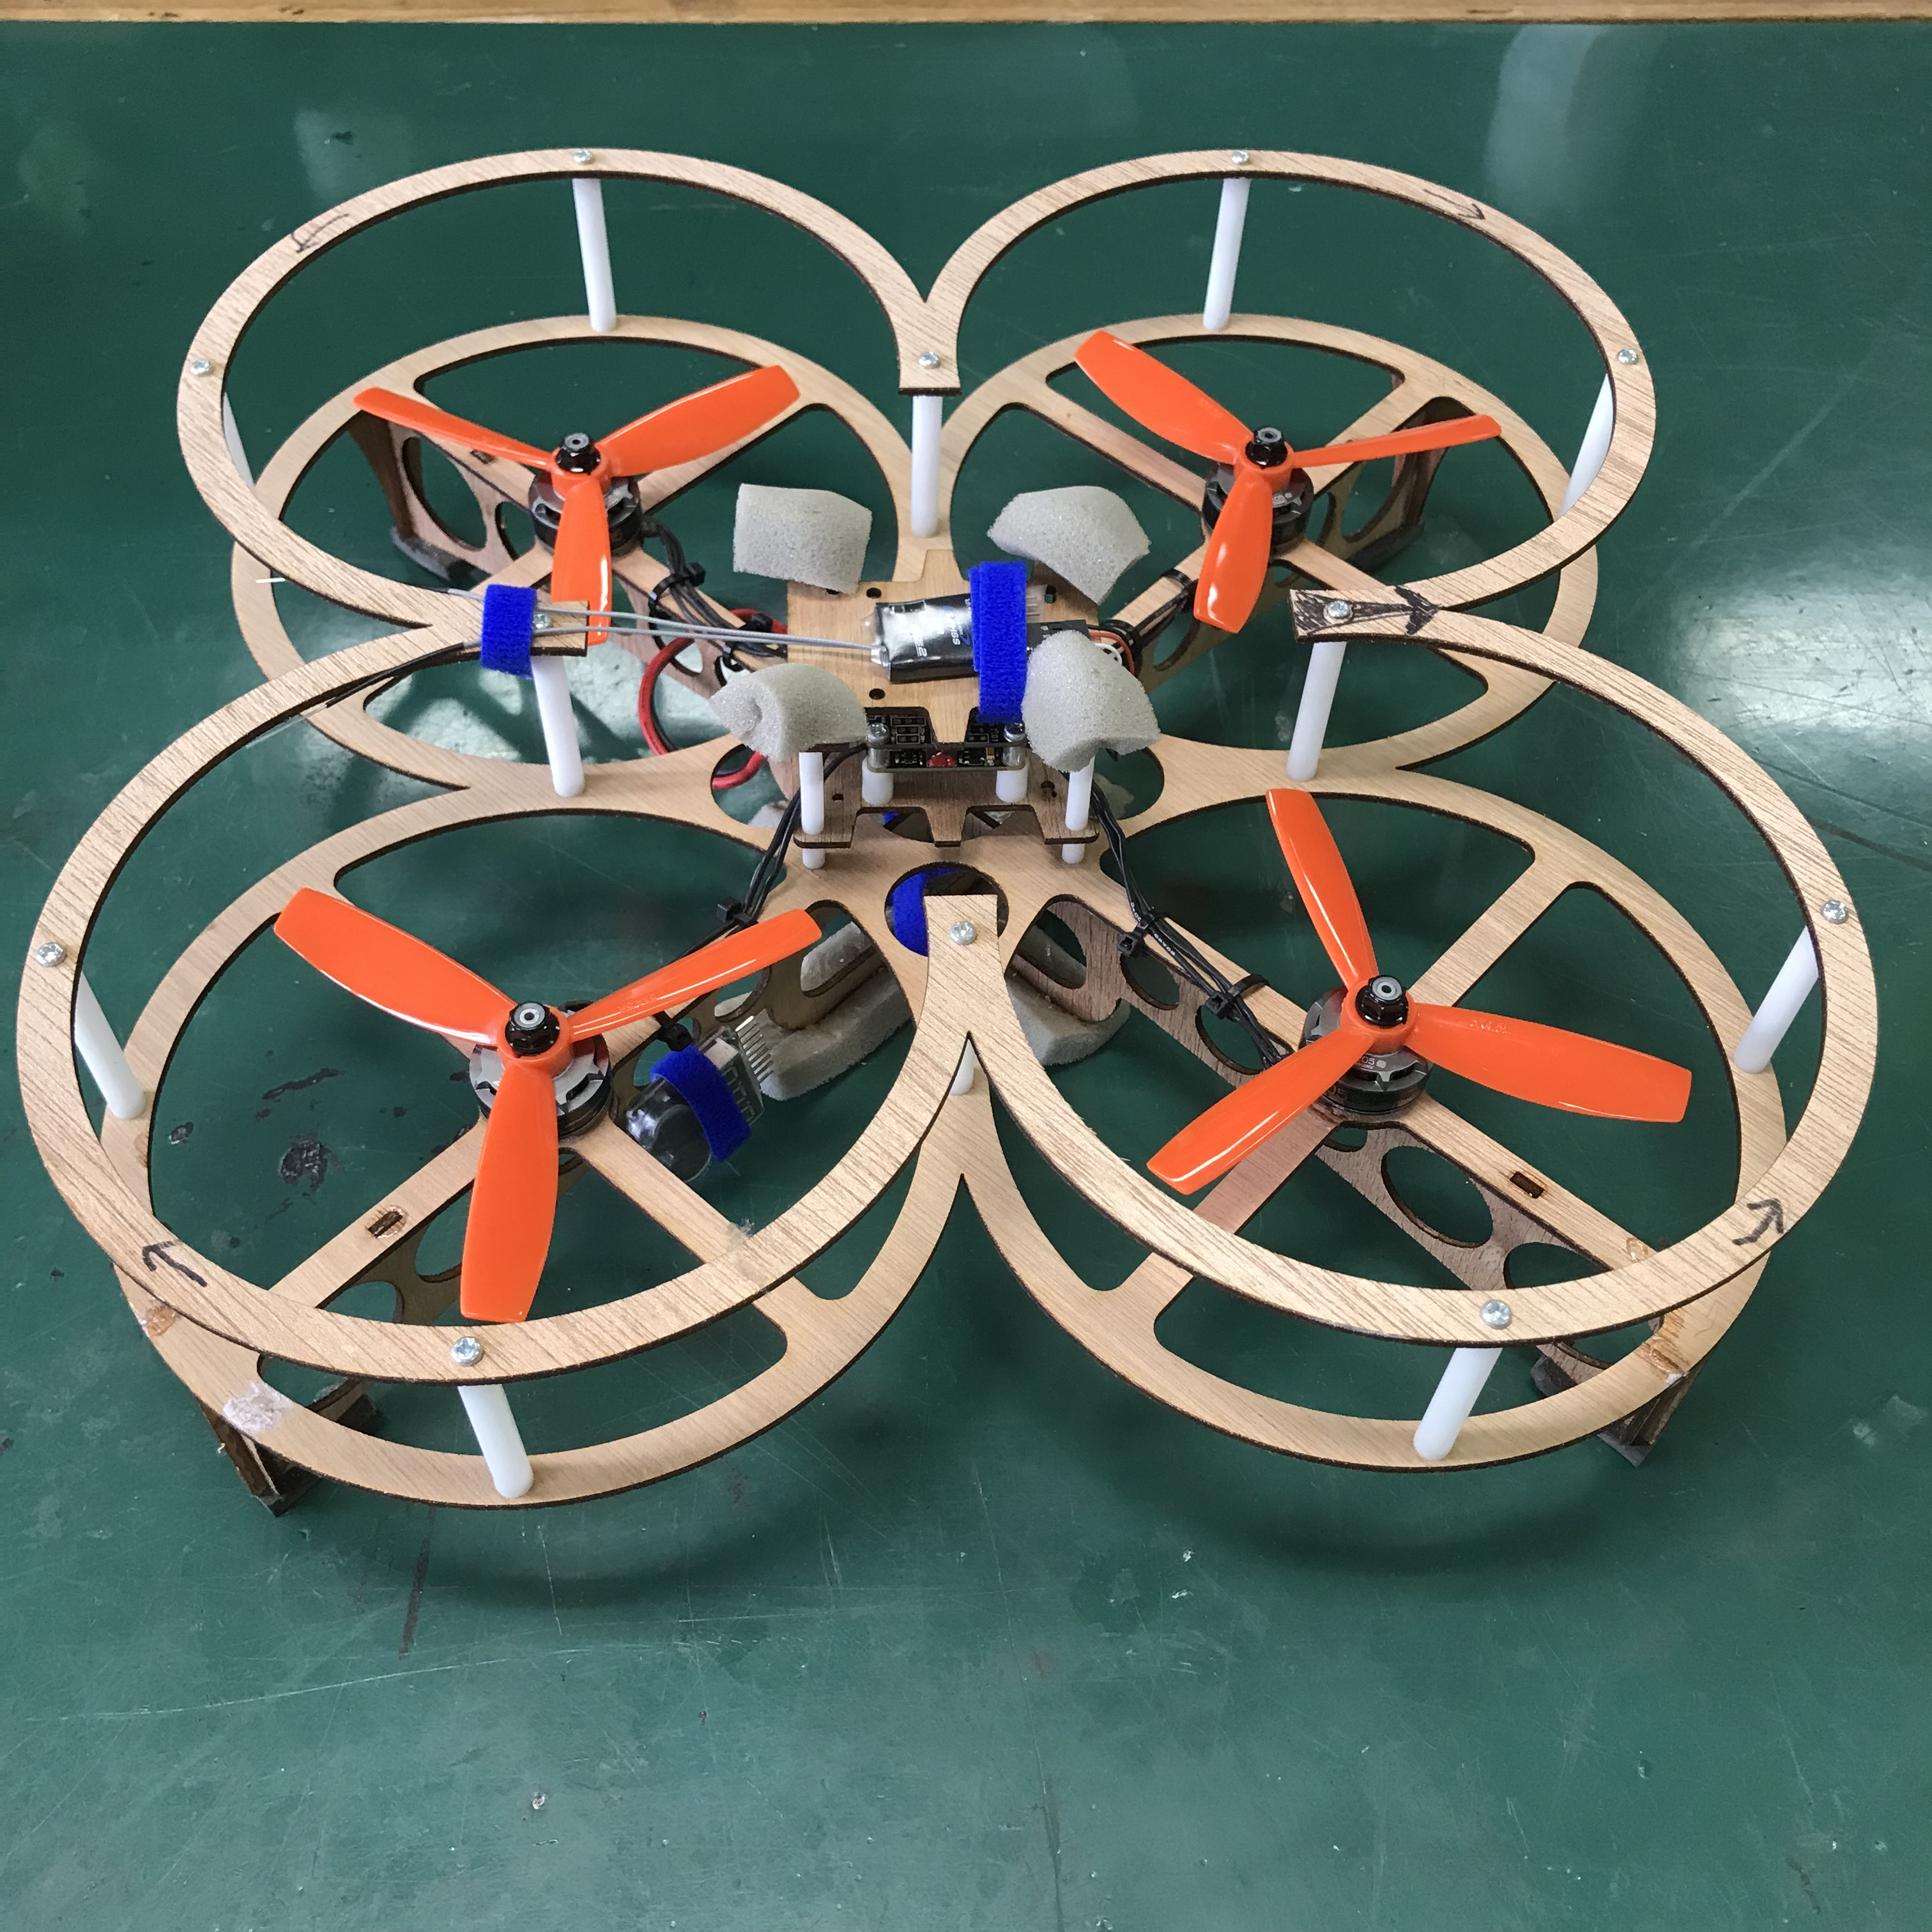
\includegraphics[width=100mm]{img/drone.jpeg}
    \end{center}
  \caption{クアッドコプター}
 \label{fig:robot}
\end{figure}

\section{研究の目的}

自動制御の課題がいくつかあり,その中に高度制御を利用した自動着陸があり,課題を達成するため高度制御について研究する.

\section{本論文の構成}
1章では,本研究の背景と簡略化した概要を示す.
2章では飛行ロボコンについて述べる.
3章ではマルチコプター運動方程式について述べる.
4章では高度制御について述べる.

5章では高度制御のシミュレーション実験について述べる.
6章で考察を述べる.
7章で最後に本実験のまとめを述べる.

\chapter{飛行ロボコン}

\section{大会ルール}
ヘリポートから飛行を開始し,ミッションエリアにてミッションを完了したのち,ヘリポートに帰還する.
大会のフィールドを図2.1に示す.

\begin{figure}[htbp]
  \begin{center}
    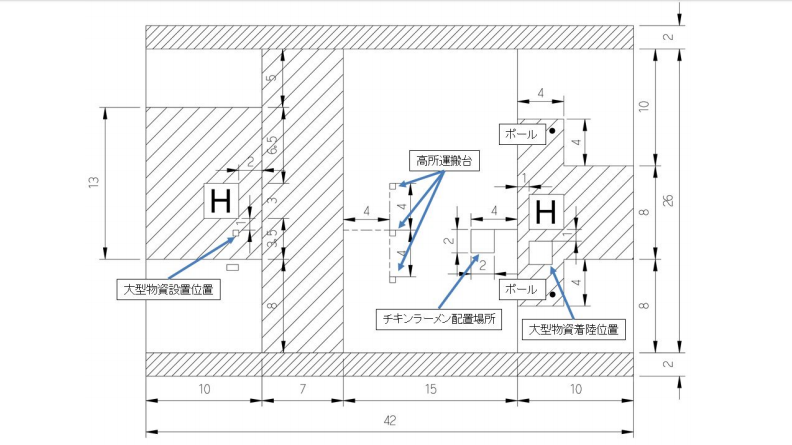
\includegraphics[width=120mm]{img/フィールド.jpg}
    \end{center}
  \caption{大会フィールド}
 \label{fig:robot}
\end{figure}

\section{機体条件}
大会に出場するための機体には以下の条件を満たさないといけない.
\begin{enumerate}
  \item 空虚重量が350g以下であり,地上補助装置との合計重量が500g以下である.
  \item 機体は自作である.
  \item 推進力として2つ以上のプロペラを搭載する機体である.
  \item 搭載する全てのプロペラ周りに安全のためにプロペラガードなどを取り付けること.

\end{enumerate}

大会に出場した機体を図2.2に示す.

\begin{figure}[htbp]
  \begin{center}
    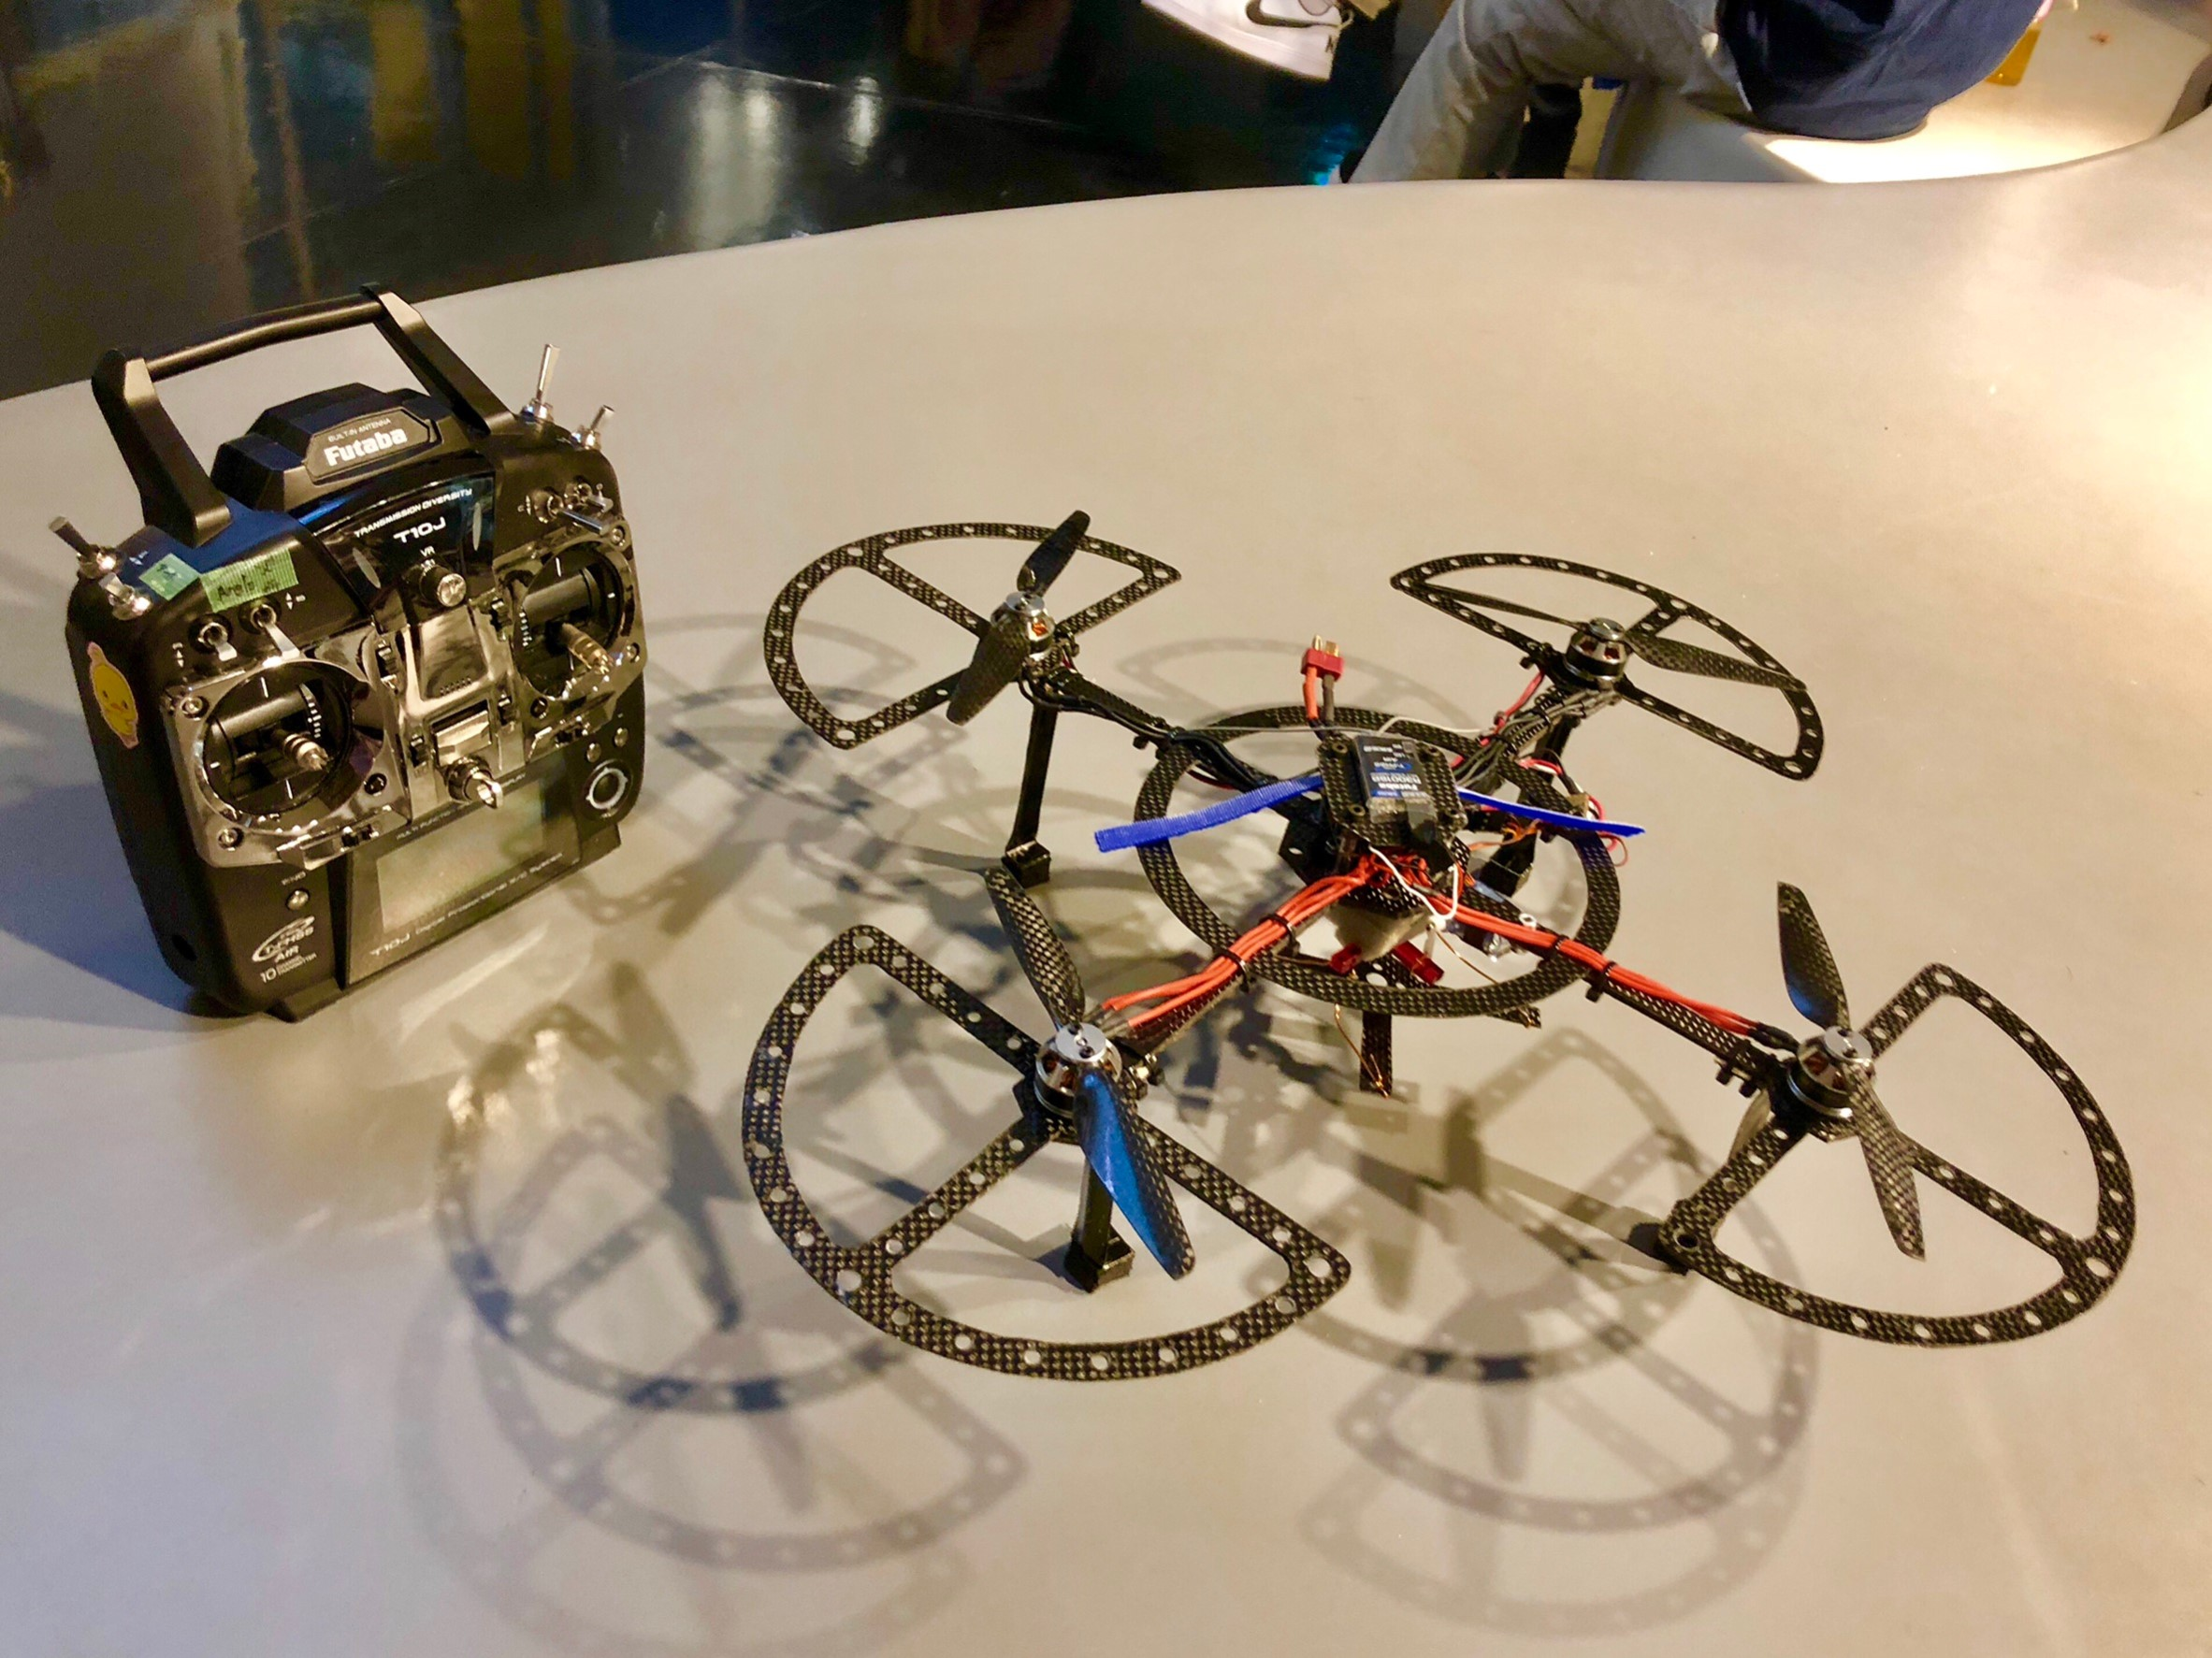
\includegraphics[width=100mm]{img/大会機.JPG}
    \end{center}
  \caption{大会機}
 \label{fig:robot}
\end{figure}

\def\MARU#1{{\rm\ooalign{\hfil\lower.168ex\hbox{#1}\hfil \crcr\mathhexbox20D}}}

我々の機体の特徴を以下に示す.
\begin{enumerate}
  \item カーボンシートを積層し軽量化かつ高い強度が得られるよう計った.カーボンを使用することで大会出場条件の350g以下になっている.
  \item 前後の進行方向の区別を目視しやすくするためにピンク色のLEDランプを使用した.そのため操縦士から見やすくなり容易に操縦できるようになる.
  \item 高所物資運搬のミッションで箱の中身を確認するのに超小型の動画撮影用のカメラを使用した.このカメラを使うことで,箱の中身を確認した後に元の位置に戻る手間が無線じゃないため電波障害が起きることがない.
  \item 操縦士がより機体を操縦できるように,機体の揺れを少なく制御を行った.
\end{enumerate}


\section{ミッション}
マルチコプター部門のミッションは以下の5種類で,\MARU{1}のミッションは競技開始と同時に開始される.\MARU{1}のミッションが終了した後,\MARU{2}~\MARU{4}のミッションの順番は問わない.\MARU{5}は最後に行うこと.

\MARU{1} 「高所物資運搬」,\MARU{2} 「大型物資運搬」,\MARU{3} 「Rocking Wings」,\MARU{4}「8の字飛行」,\MARU{5}「自動離着陸」

予選と決勝におけるミッション
予選では「高所物資運搬」「8の字飛行」の2つのみ挑戦をが認められる.決勝では全てのミッションへの挑戦が認められる.

\section{大会結果}
大会は11チーム出場し,我々の予選結果は840点を獲得し2位となり決勝へと駒を進めた.
決勝は4チーム勝ち上がった.
決勝で我々が挑戦したミッションは予選の「高所物資運搬」と「8の字飛行」に加えて,「大型物資運搬」に挑戦した.
3つのミッションに挑戦した結果,1925点獲得し2位と500点近くの差をつけて優勝することができた.

\section{大会の勝因}

我々の大会の勝因を以下に示す.
\begin{enumerate}
  \item フレームすべてをカーボンにしたことで軽量で高い強度が得られた.またフレームの厚みを変えたことで軽くなった.
  \item 高所物資運搬のミッションにチキンラーメンを箱の中に入れるためのサーボ機構が安定していた.そのため機体に与える影響が少なくなった.
  \item 戦略がよく高得点が出た.自動を含むミッションに挑戦しなかったため電波障害が起きることがなかった.
  \item 制御の安定性があったため機体の揺れが少なく,操縦しやすくなっていた. 
  \item 操縦士の技量があり,緊張もせずに挑むことができた.
\end{enumerate}

\section{大会の反省点}

我々の大会の反省点を以下に示す.
\begin{enumerate}
  \item 大会ルールの確認不足.大会で使用できるバッテリーのセル数は2セルなのだが確認不足だったため3セルで出場しようとしてしまい,会場の近くのお店に急いで買い出しに行くこととなった.
  \item 大会前の準備期間のスケジュールがチーム内で全員が揃うことが少なかった.
\end{enumerate}








\chapter{マルチコプターの運動方程式}

\section{マルチコプターの上下運動に関する微分方程式(運動方程式)}

\begin{eqnarray}
m\ddot{y}=T-mg
\end{eqnarray}


\begin{eqnarray}
\dot{v}=\ddot{y}=\frac{T-mg}{m}\\
\end{eqnarray}

y:マルチコプターの高度[m]

T:4つのプロペラの推力[N]

m:マルチコプターの質量[kg]

v:上昇・下降速度[m/s]


\section{モーターの回転運動に関する微分方程式(一次遅れモデル)}

\begin{eqnarray}
τ\dot{ω}+ω=ku
\end{eqnarray}

\begin{eqnarray}
\dot{ω}=\frac{ku-ω}{τ}\\
\end{eqnarray}

ω:モーターの角速度[rad/s]

τ:モーターの時定数[s]

\begin{eqnarray}
k:モーターのゲイン[\frac{rad/s}{V}]
\end{eqnarray}

\section{角速度とプロペラの推力との関係}

%\[
%  x = (\frac{a}{b}) %単純に括弧で囲った場合
%\]
%\[
%  x = \left( \frac{a}{b} \right) %\left( \right)で囲んだ場合
%\]

\begin{eqnarray}
T=\frac{Gω^2}{{1-\frac{64}{9D^2}}{(\frac{v}{ω})^2}}
\end{eqnarray}

T:推力

G:推力係数

ω:プロペラ角速度

D:プロペラ直径

v:上昇・下降速度

プロペラ直径が6インチ
D=0.1524mとすると,
上式は

\begin{eqnarray}
T=\frac{Gω^2}{{1-306}{(\frac{v}{ω})^2}}
\end{eqnarray}

上昇・下降速度vはωに対して非常に小さいので
\begin{eqnarray}
T\fallingdotseq Gω^2
\end{eqnarray}

として良い.


シミュレーションのためにマルチコプターの質量m=0.65kg,モーターに与える電圧eと回転数Nの関係は,
\begin{eqnarray}
N=K_V \large{e}  [rpm]
\end{eqnarray}

我々の使用しているモーターは
\begin{eqnarray}
K_V =2600 [rpm/V]
\end{eqnarray}


単位変換すると


\begin{eqnarray}
ω=K_V' \large{e}   [rad/s]
\end{eqnarray}

\begin{eqnarray}
K_V' =\frac{K_V・2π}{60} = \frac{πK_V}{30} \fallingdotseq 272.3
\end{eqnarray}

3.9式と3.16式からホバリングに必要な電圧を電池の半分の電圧5Vを考えGを求める.
※モーターとプロペラ4個の推力がマルチコプターの重量に等しくなる.


\begin{eqnarray}
mg=4T
\end{eqnarray}ということになる.





\chapter{高度制御}

高度センサーで高度を計測して,制御する.センサーの性能を測定した.いかにその結果を示す.

今回使用した超音波センサーを図4.1に示す.
\begin{figure}[htbp]
  \begin{center}
   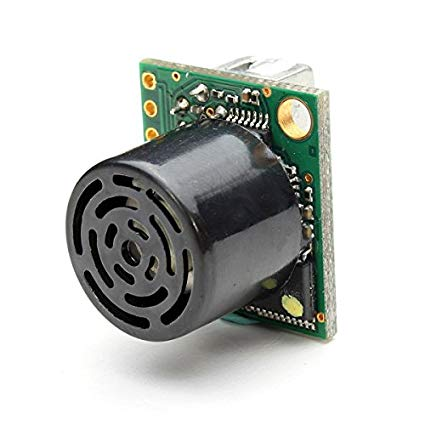
\includegraphics[width=100mm]{img/超音波センサー.jpg}
    \end{center}
  \caption{超音波センサー}
 \label{fig:ensyu3tex}
\end{figure}


\section{超音波センサーの性能確認}

以下に実験手順を示す.

\begin{enumerate}
  \item 距離と出力の確認.
アクリル板を少しずつずらして,距離と出力の関係を確認した.

\begin{figure}[htbp]
  \begin{center}
   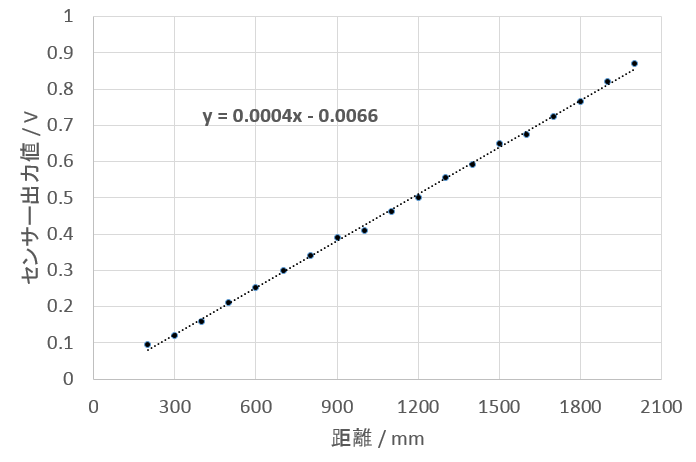
\includegraphics[width=150mm]{img/距離と出力.jpg}
    \end{center}
  \caption{超音波センサーの距離と出力の関係}
 \label{fig:ensyu3tex}
\end{figure}

図4.2より,距離に応じてセンサーの出力値が比例していることがわかる.

  \item 検知範囲の確認.

センサーの検知範囲を確認した.

\begin{figure}[htbp]
  \begin{center}
   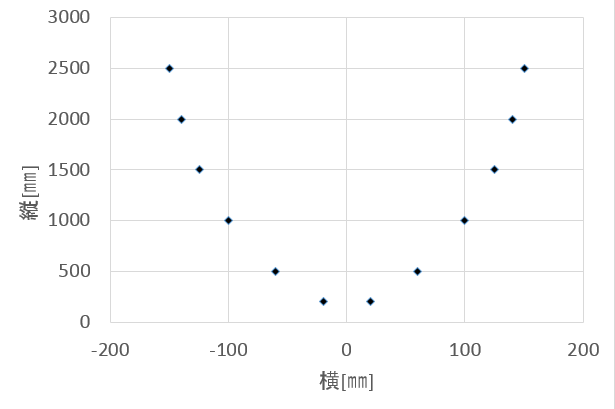
\includegraphics[width=150mm]{img/検知範囲.png}
    \end{center}
  \caption{超音波センサーの検知範囲}
 \label{fig:ensyu3tex}
\end{figure}

図4.3より超音波センサーの音波は広範囲に広がって検知している.
超音波センサーの性能を確認することができた.
\end{enumerate}




\chapter{高度制御のシミュレーション実験}
制御性能をシュミレーションで確認する.

Pythonによって製作された制御シミュレーションCADを用いて,PID制御の比例ゲイン$K_P$,積分ゲイン$K_I$,微分ゲイン$K_D$に値を入れてシミュレーションを模擬実験する.

\section{PID制御}
偏差(目標値と現在値の差)に比例して制御量が増える比例制御(P),偏差がある状態が長時間続くにつれ制御量が増えていく積分制御(I),偏差が急激な変化をするほど制御量が増える微分制御(D)を組み合わせた基本的な制御手法である.
ブロック線図を図5.1に示す.

\begin{figure}[htbp]
  \begin{center}
   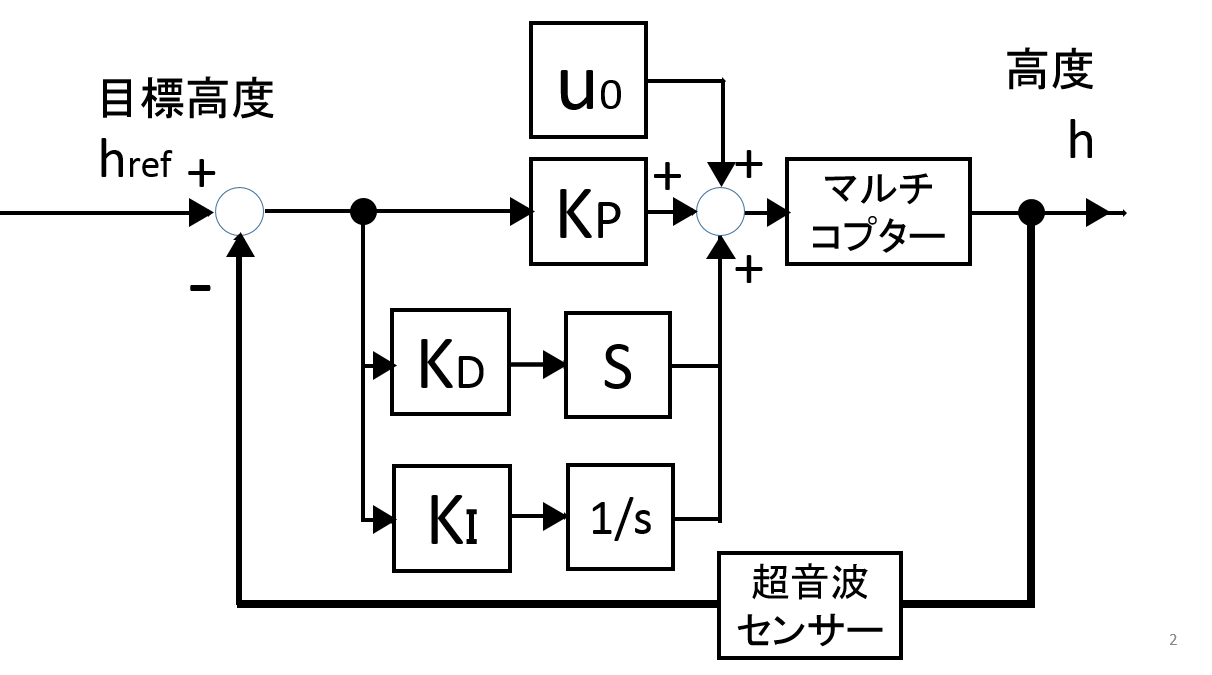
\includegraphics[width=150mm]{img/ブロック線図.png}
    \end{center}
  \caption{ブロック線図}
 \label{fig:ensyu3tex}
\end{figure}


目標高度 $h_{ref}$

実際の高度 h

誤差 e

とすると,

\begin{eqnarray}
e=h_{ref}-h
\end{eqnarray}

PID制御とは,制御入力uを次式で与える制御方式である.

\begin{eqnarray}
u=K_P\large{e}+K_D \large{e}+K_I\int\large{e}dt+u_0
\end{eqnarray}

\begin{eqnarray}
eの微分 \dot{e} とeの積分∫\large{e}dtについては,実際のプログラムでは制御周期をΔtとして
\end{eqnarray}


\begin{eqnarray}
\dot{e}\fallingdotseq \frac{ e_n-e_{(n-1)}}{Δt}\\
\end{eqnarray}

\begin{eqnarray}
∫edt \fallingdotseq \sum e
\end{eqnarray}


ここで
$K_P$ :比例ゲイン 

$K_D$ :微分ゲイン

$K_I$ :積分ゲイン



\begin{enumerate}
  \item 比例制御のみの結果を図5.2に示す.
比例制御だけでは発散して,高度制御ができないことがわかる.


  \item 比例制御と微分制御の実験を行った結果を図5.3に示す.
微分制御を加えたことで,安定するが目標値に一致しないことがわかる.


  \item 積分制御を使った結果を図5.4に示す.
積分制御を加えたことで,目標値に一致していることがわかる.

\begin{figure}[htbp]
  \begin{center}
   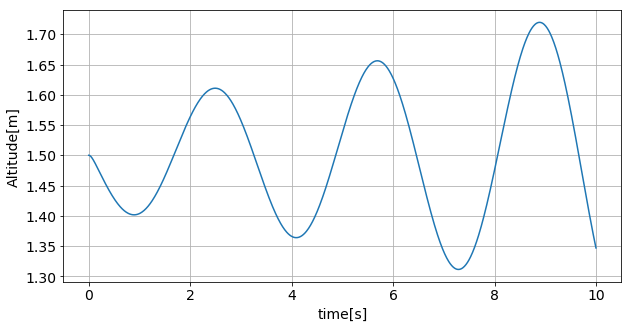
\includegraphics[width=150mm]{img/発散.jpg}
    \end{center}
  \caption{比例制御のみの高度結果}
 \label{fig:ensyu3tex}
\end{figure}

\begin{figure}[htbp]
  \begin{center}
   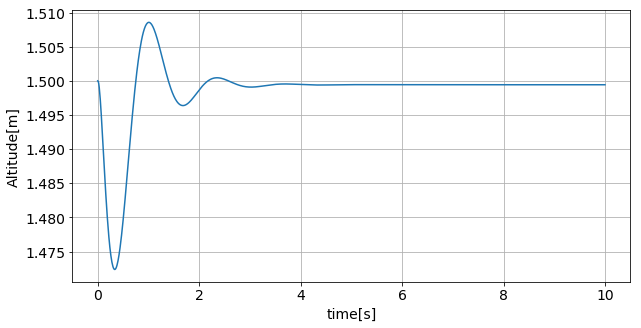
\includegraphics[width=150mm]{img/PD.jpg}
    \end{center}
  \caption{比例制御,微分制御の高度結果}
 \label{fig:ensyu3tex}
\end{figure}

\begin{figure}[htbp]
  \begin{center}
   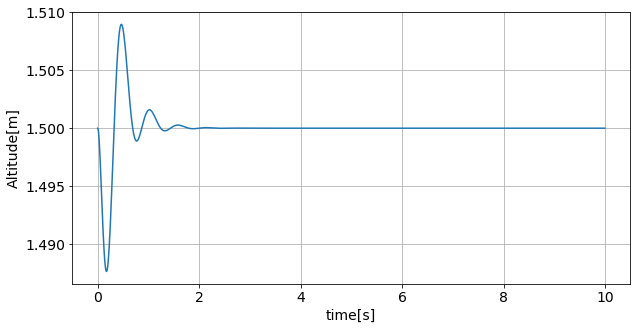
\includegraphics[width=150mm]{img/PIDbest.jpg}
    \end{center}
  \caption{比例制御,微分制御,積分制御の高度結果}
 \label{fig:ensyu3tex}
\end{figure}

\end{enumerate}


\chapter{考察}
図5.2より比例制御だけではマルチコプターが上下に発散して,高度制御ができないことがわかる.次に図5.3より比例制御に微分制御を加えたことで,安定するが目標値に一致しないことがわかる.最後に図5.4より比例制御と微分制御に積分制御を加えたことで,目標値に一致していることがわかる.これらの図より,初めに落ちてしまっている.これは1メモリ0.01mなので実際には約10mmしか落ちないので,あまり影響がないと考える.

%\chapter{リフトについて}

\section{要求される仕様}
\subsection{ロボコンのルール}
今年度のロボコンのタイトルは「ロボット・ニューフロンティア」で,新大陸の開拓をテーマとしている.今回の競技フィールドを(図\ref{fig:field})に示す.新大陸では,スタート地点から運んできたプラスティック製段ボールの箱(図\ref{fig:plabox})を高く積み上げる課題が課されている.港町と島,島と新大陸までの間の海にはロボットは接地してはならない.積み上げロボットはスタート地点と島に置いてあるプラスティック製段ボールを取りに行き高台に小さい砦を積み上げる.高台の砦が完成後,新大陸に向かい丘に砦を完成させる.これを2チームでいかに高く積み上げるかを競い合う競技となっている.

\begin{figure}[htbp]
  \begin{center}
    \includegraphics[width=130mm]{img/field.png}
    \end{center}
  \caption{競技フィールド}
 \label{fig:field}
\end{figure}

\subsection{我々の戦略}
プラスティック製段ボールの積み方を(図\ref{fig:tumikata})に示すように,同じ数の箱を積み上げる場合,箱の長手方向を縦向きにして積み上げる方が高く積み上げられる.よってリフトの可動高さを400[mm]になるよう設計,製作した.だが,長手方向を縦向きにすることで重心位置が高くなり,底面積が減るため落下時にバランスが崩れ,倒れる恐れがあるため注意する必要がある.


\begin{figure}[htbp]
  \begin{center}
    \includegraphics[width=90mm]{img/tumikata.png}
    \end{center}
  \caption{プラスティック段ボールの積み方}
 \label{fig:tumikata}
\end{figure}

\begin{figure}[htbp]
  \begin{center}
    \includegraphics[width=100mm]{img/plabox.png}
    \end{center}
  \caption{プラ段の箱の仕様}
 \label{fig:plabox}
\end{figure}




\section{動作原理}
積込ロボットの前面にリフトが搭載されている(図\ref{fig:lift}).
リフト中央下部に設置されているモータによってスプロケットが回転し,チェーン駆動をする.
リフト上端と下端に設置してあるリミットセンサには通過型フォトインタラプタを使用している.リミットセンサは距離が400[mm]になるように位置が調整されているため,箱を400[mm]の高さに持ち上げることが出来る.



\begin{figure}[htbp]
  \begin{center}
    \includegraphics[width=80mm]{img/lift.jpg}
    \end{center}
  \caption{積み込みロボットのリフト}
 \label{fig:lift}
\end{figure}

\section{回路構造}
リフトに関わるロボットのシステムブロック線図は図\ref{fig:roboblock}のようになっている.arduinoは図\ref{fig:arduino}にあるようなarduinoMegaを使用した.このarduinoはUSBホストシールド(図\ref{fig:USBhs})を介したBluetoothでの通信でコントローラの信号を受け取る.コントローラでの操作と上下リミットセンサの信号を受け取り,図\ref{fig:motordrive}のモータドライバに指示を送り,リフト駆動用のモータを制御している.モータドライバはarduinoから正転,逆転,PWM値を受け取り,モータに最大12[V]の電圧を印加する.

\begin{figure}[htbp]
  \begin{center}
    \includegraphics[width=120mm]{img/roboblock.png}
    \end{center}
  \caption{ロボットのシステムブロック線図}
 \label{fig:roboblock}
\end{figure}

\begin{figure}[htbp]
  \begin{center}
    \includegraphics[width=100mm]{img/arduinoMega.JPG}
    \end{center}
  \caption{arduino Mega}
 \label{fig:arduino}
\end{figure}

\begin{figure}[htbp]
  \begin{center}
    \includegraphics[width=100mm]{img/USBhs.JPG}
    \end{center}
  \caption{USBホストシールド}
 \label{fig:USBhs}
\end{figure}

\begin{figure}[!htbp]
  \begin{center}
    \includegraphics[width=90mm]{img/motordrive.JPG}
    \end{center}
  \caption{モータドライバ}
 \label{fig:motordrive}
\end{figure}

\section{使用部品}
使用した部品の詳細を以下の表\ref{tab:parts}に示す.

\begin{table}[!htb]
 \begin{center}
  \caption{搭載部品の型番とメーカ}
  \begin{tabular}[htbp]{|c|c|c|}
   \hline
   製品名&型番&メーカ \\
   \hline
   arduino&ArduinoMega&Arduino SRL\\
   \hline
   USBホストシールド&BOO6J4GOOO&サインスマート\\
   \hline
   DCモータ&組み合わせモータ323726&マクソン\\
   \hline
   コントローラ&DUALSHOCK3&ソニー\\
   \hline
   モータドライバ&-&夢考房\\
   \hline
   リミットセンサ&CNZ1023&パナソニック\\
   \hline
  \end{tabular}
  \label{tab:parts}
 \end{center}
\end{table}

%
\chapter{位置制御}位置制御とは,制御対象の現在位置を何らかのセンサなどで検出し,目標の位置になるようにフィードバック制御を行うことである.

\section{位置検出}今回のリフトのようにモータを動力とする位置制御をする際は,ロータリーエンコーダでモータの回転角度を検出し,ギヤ比やスプロケット半径から計算して制御対象の位置を特定する.このように,位置制御を行う際は位置を直接取得できるセンサを使用して,その値をフィードバックするのが一般的である.

\section{制御手法}
制御には主に以下のような手法が使われる.

\subsection{PID制御}目標値と現在値の差のことを偏差という.偏差に比例して制御量が増える制御を比例制御(P)といい,比例定数Kpは比例ゲインと呼ばれる.比例制御では偏差が0になると制御量が0になるため,いつまでたっても偏差が残り続ける事がある.この残留偏差をなくすため,偏差を時間で積分したものをKi倍して制御量に加えると,残留偏差のある時間が長いほど制御量が増えていき最終的に偏差が無くなる.これを積分制御(I)といい,Kiは積分ゲインと呼ばれる.偏差が急激な変化をする動き始めと動き終わりには,偏差を微分した値が大きくなる.微分に比例して制御量を大きくすると機敏な動作をするようになり,早く目標値に到達する.これを微分制御(D)といい,この比例定数Kdは微分ゲインと呼ばれる.これらP,I,D制御を組み合わせた基本的な制御手法がPID制御(図\ref{fig:PID})である.

\begin{figure}[htbp]
  \begin{center}
    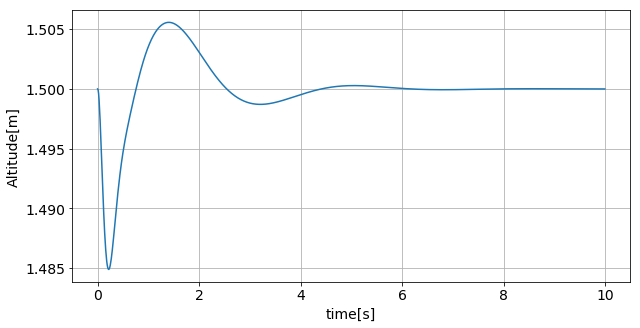
\includegraphics[width=135mm]{img/PID.png}
    \end{center}
  \caption{PID制御のブロック線図}
 \label{fig:PID}
\end{figure}

\subsection{極配置法}システムは式(\ref{eq:joutai})のような状態方程式という形で表すことが出来る.状態方程式はシステムへの入力$u$,システムからの出力$y$,システムの状態量$x$の関係を表した方程式である.システムは伝達関数で表され、その分母は特性方程式という.特性方程式の解は極と呼ばれ,その値によって応答速度や行き過ぎ量などの特性が変化する.状態方程式で表されたシステムに対し,状態量$x$に一定の値(ゲイン)を掛けて入力にフィードバックすることで極を変化させることができる.極を望ましい値に設定するフィードバックゲインを探る方法を極配置法という.

\begin{eqnarray}
\begin{array}{l}
\dot{x}=\bm{A}x+\bm{B}u\\
y=\bm{C}x+\bm{D}u
\end{array}
\label{eq:joutai}
\end{eqnarray}


%\chapter{位置センサレス位置制御}

\section{センサレスの有効性}上述したように今回のリフトのような位置制御を行う場合,通常,モータの回転角度を検出するロータリーエンコーダを使用して移動量を算出する.しかし,ロータリーエンコーダを使用するにはそれ専用の取付部を新しく設計し取り付けるか,既にロータリーエンコーダと一体化しているモータを購入し使用する必要がある.ロータリーエンコーダを取り付けるにはブラケットや軸継手が必要になり,さらに取付精度も要求される.一体化されたモータなら精度は確保されているが,一般に高価である.
このように,ロータリーエンコーダを後から取り付ける場合は金銭的,時間的にコストがかかる場合が多い.今回提案する位置制御はロボットに取り付ける専用のパーツを使わないため,実現できればそれらのコストを減らすことができる.

\section{センサレス制御の方法}
モータの電流,電圧,回転速度には相関があり,二つの値が定まると残りの一つの値も定まる.電圧の値は操作量なので既知であるため,電流の値が取得できれば,モータの回転速度を求め,それを積分して回転角度を求め,そこから移動量を算出することが出来る.必要なものは電流センサを使った電流計測回路のみなので,ロータリーエンコーダを使うよりも後付けを簡単に行うことができる.

\subsection{制御対象のモデル}
リフトの簡略モデルを図\ref{fig:liftModel}に示す.リフトの運動方程式は式(\ref{eq:lift})のようになる.

\begin{figure}[htbp]
  \begin{center}
    \includegraphics[width=170mm]{img/liftModel.png}
    \end{center}
  \caption{リフトの簡略モデル}
 \label{fig:liftModel}
\end{figure}

\begin{eqnarray}
m\dot{v}=\frac{T}{r}-mg\\
\label{eq:lift}
\end{eqnarray}

式(\ref{eq:lift})をトルクについて変形すると,式(\ref{eq:lift2})のようになる.

\begin{eqnarray}
T=rm(\dot{v}+g)\\
\label{eq:lift2}
\end{eqnarray}

モータ回路の簡略モデルを図\ref{fig:circuitmodel}に示す.モータの運動方程式は式(\ref{eq:motor})のようになる.

\begin{figure}[htbp]
  \begin{center}
    \includegraphics[width=150mm]{img/circuitmodel.png}
    \end{center}
  \caption{モータ回路簡略モデル}
 \label{fig:circuitmodel}
\end{figure}

\begin{eqnarray}
RI+K{\omega}=c\\
J\dot{\omega}+\frac{D}{n}{\omega}-\frac{T}{n}=KI
\label{eq:motor}
\end{eqnarray}

モータの回転数と歯車比,スプロケット半径との関係は式(\ref{eq:rote-v})で表される.

\begin{eqnarray}
{\omega}=\frac{v}{n}r
\label{eq:rote-v}
\end{eqnarray}

リフトの上昇速度を状態量に,電流値を観測方程式とする状態方程式を立てる.式(\ref{eq:lift}),式(\ref{eq:motor})より,リフトの状態方程式は式(\ref{eq:system})のようになる.

\begin{eqnarray}
%\begin{array}{l}
\dot{v}=-\frac{RD+K^2}{RJ+r^{2}m/n^2}v+\frac{KRn}{RJn^{2}+r^{2}m}u-\frac{g}{Jn^{2}/r^{2}m+1}\\
I=-\frac{Kn}{Rr}v+\frac{1}{R}u
%\end{array}
\label{eq:system}
\end{eqnarray}

リフトの状態方程式の観測方程式を変形し,リフトの速度を電流と電圧で表すと式(\ref{eq:rote-I-u})のようになる.
\begin{eqnarray}
v=-\frac{Rr}{Kn}I-Ru
\label{eq:rote-I-u}
\end{eqnarray}

式(\ref{eq:rote-I-u})には質量$m$が含まれていない.よって速度推定はリフトの荷重によって影響されないと考えられる.

\subsection{制御系設計}ブロック線図を図\ref{fig:burokkusennzu}に示す.

\begin{figure}[htbp]
  \begin{center}
    \includegraphics[width=130mm]{img/burokkusennzu.png}
    \end{center}
  \caption{ブロック線図}
 \label{fig:burokkusennzu}
\end{figure}

リフトには,目標値と現在値の偏差に比例した値を入力する比例制御を行っている.通常の位置制御であればリフトの位置を直接検出してフィードバック制御を行う.しかし今回のセンサレス制御では位置を検出できない.そのため,電流センサから得た電流と入力の電圧から速度測定器でリフトの移動速度を求め,それを積分した値を現在値としてフィードバックする.速度推定器は式(\ref{eq:speed})で表される.

\begin{eqnarray}
v=-\frac{Rr}{Kn}i+\frac{R^2r}{Kn}u
\label{eq:speed}
\end{eqnarray}

速度測定器で算出した移動速度は実際のリフトの移動速度とは異なる可能性がある.


%\chapter{実験}
\section{シミュレーション}
シュミレーションを利用して,設計した制御系の性能を確認する.

\subsubsection{シミュレーションソフト}
シミュレーションには数値計算ソフト「Scilab」に付属しているビジュアルモデリングソフト「Xcos」を使用する.Xcosで組み立てたブロック線図を図\ref{fig:blockXcos}に示す.この際、リフトにかかる電圧の絶対値の最大は実際と同じく12[v]に制限した.

\begin{figure}[htbp]
  \begin{center}
    \includegraphics[width=150mm]{img/blockXcos.png}
    \end{center}
  \caption{Xcosで組み立てたブロック線図}
 \label{fig:blockXcos}
\end{figure}

\subsubsection{シミュレーション結果}
シミュレーションの結果を図\ref{fig:sim}に示す.

\begin{figure}[htbp]
 \begin{center}
    \includegraphics[width=150mm]{img/sim.bmp}
    \end{center}
  \caption{入力した目標値による電圧と位置の時間変化}
 \label{fig:sim}
\end{figure}

\subsubsection{荷重の影響}
リフトは箱を持つ個数により荷重が変化する,荷重の影響を見るためリフトの質量の値を2倍にした.その際のシミュレーション結果を図\ref{fig:sim4}に示す.

\begin{figure}[htbp]
 \begin{center}
    \includegraphics[width=150mm]{img/sim4.bmp}
    \end{center}
  \caption{荷重による影響}
 \label{fig:sim4}
\end{figure}

荷重によって電圧は2倍になったが,現在値の最終値に変化はなかった.

\subsubsection{測定誤差の影響}
実際に電流を測定した時にはノイズがあると考え,ノイズの影響を見るため電流の値に1[A]の誤差を加えてシミュレーションした.その結果を図\ref{fig:sim5}に示す.

\begin{figure}[htbp]
 \begin{center}
    \includegraphics[width=150mm]{img/sim5.bmp}
    \end{center}
  \caption{測定誤差の影響}
 \label{fig:sim5}
\end{figure}

電流の値に誤差があると,実際のリフトの速度と推定する速度にずれが生じることが分かった.

\subsubsection{測定ノイズの影響}
実際に電流を測定した時にはノイズがあると考え,ノイズの影響を見るため電流の値を分散が1[A]の正規分布になるようにした.その際のシミュレーション結果を図\ref{fig:sim2}に示す.

\begin{figure}[htbp]
 \begin{center}
    \includegraphics[width=150mm]{img/sim2.bmp}
    \end{center}
  \caption{測定ノイズの影響}
 \label{fig:sim2}
\end{figure}

電圧のグラフが激しく振動している為,塗りつぶされて見える.これは電流のノイズの影響だと考えられるが,ノイズの平均値が0ならば現在位置に影響はなかった.

\section{検出誤差の確認}
電流センサが検出する電流と実際に流れている電流に誤差があると,リフトの速度推定にも誤差が生じてしまい,時間が経つにつれリフトの位置がずれていってしまう.ここでは電流センサで検出した値がどれだけの測定誤差を持つのか確認する.

\subsubsection{使用機器}
電流センサを内蔵したモータドライバを使用した.使用したモータドライバを図\ref{fig:currentDriver}に示す.使用した機器一覧を表\ref{tab:partsCurrent}に示す.

\begin{figure}[H]
 \begin{center}
    \includegraphics[width=75mm]{img/currentDriver.JPG}
    \end{center}
  \caption{電流センサ内臓モータドライバ}
 \label{fig:currentDriver}
\end{figure}

\begin{table}[H]
 \begin{center}
  \caption{搭載部品の型番とメーカ}
  \begin{tabular}[htbp]{|c|c|c|}
   \hline
   製品名&型番&メーカ \\
   \hline
   arduino&ArduinoUno&Arduino SRL\\
   \hline
   DCモータ&組み合わせモータ323726&マクソン\\
   \hline
   電流センサ内臓モータドライバ&MD01B&Pololu\\
   \hline
   テスター&VOAC86&IWATU\\
   \hline
  \end{tabular}
  \label{tab:partsCurrent}
 \end{center}
\end{table}

\subsubsection{計測方法}
\begin{enumerate}
\renewcommand{\labelenumi}{\arabic{enumi}).}
\item arduinoで,モータに常に電圧を12[v]印加するように,電流センサの値を1ミリ秒ごとに取得するようにプログラミングする.
\item 10秒以上データを記録したら,電流の平均値と分散を算出する.突入電流といい,モータに電圧を印加した直後は大きな電流が瞬間的に流れるため,しばらくたった定常状態の値を計算に使用する.
\item テスターを用いて実際の電流を計測する.
\item 電流センサでの平均値とテスターでの計測値の差を求め,ノイズの平均値とする.
\end{enumerate}

\subsubsection{電流計測}
電流を計測した結果を図\ref{fig:currentMeasurement}に示す.

\begin{figure}[H]
 \begin{center}
    \includegraphics[width=150mm]{img/currentMeasurement.png}
    \end{center}
  \caption{電流の時間変化}
 \label{fig:currentMeasurement}
\end{figure}

検出した電流の平均は0.575[A],ノイズの分散は0.016[A],テスターでの計測結果は0.232[A]となった.よってノイズの平均は0.343[A]となった.
\\
モータに印加する電圧を負にして,逆転させた場合の計測結果を図\ref{fig:currentMeasurement3}に示す.

\begin{figure}[H]
 \begin{center}
    \includegraphics[width=150mm]{img/currentMeasurement3.png}
    \end{center}
  \caption{電流の時間変化}
 \label{fig:currentMeasurement3}
\end{figure}

検出した電流の平均は0.027[A],ノイズの分散は0.002[A]となった.よってノイズの平均は -0.205[A]となった.
%オシロの図とメーカ名もいるので書いといて
正転時と逆転時に電圧の違いが表れたが,arduinoのAD変換器に原因がある可能性を考え,オシロスコープで電流センサから出力される電圧を直接観察した.その結果を図\ref{fig:osiro_0},図\ref{fig:osiro_seiten},図\ref{fig:osiro_gyakuten}に示す.

\begin{figure}[htbp]
 \begin{center}
    \includegraphics[width=100mm]{img/osiro_0.jpg}
    \end{center}
  \caption{無回転時の電圧}
 \label{fig:osiro_0}
\end{figure}

\begin{figure}[htbp]
 \begin{center}
    \includegraphics[width=100mm]{img/osiro_seiten.jpg}
    \end{center}
  \caption{正転時の電圧}
 \label{fig:osiro_seiten}
\end{figure}

\begin{figure}[htbp]
 \begin{center}
    \includegraphics[width=100mm]{img/osiro_gyakuten.jpg}
    \end{center}
  \caption{逆転時の電圧}
 \label{fig:osiro_gyakuten}
\end{figure}







%図入れといて
オシロスコープでの観察でも電圧の値に差がみられた.


\chapter{おわりに}
\section{結論}
高度制御について超音波センサーの性能確認の実験とPID制御を利用したシミュレーション実験を行った.
PID制御をすることにより高度制御を成功した.


\section{今後の課題}
制御し始めに少しだけ落ちてしまっているため更に研究が必要であると考えられる.


また,PID制御を実機に加えて実験をする必要があると考える.
%シミュレーションを使用して,センサレス制御は可能であることを確認することができた.実験に使用したモータドライバには特性があり,正転と逆転時に異なる電流値を出力することが分かったため,この制御を実際のリフトに適用する際には,電流センサのノイズによって引き起こされる速度推定誤差とモータのモデル化誤差を何らかの方法で補正して解決する必要があると考えられる.

\begin{thebibliography}{8}
\bibitem{ob} 和栗雄大郎,模型飛行機の科学,養賢堂,2005/07/01

%\bibitem{ob} 熊谷正朗,状態フィードバックとオブザーバ,www.mech.tohoku-gakuin.ac.jp\slash{}rde\slash{}contents\slash{}course\slash{}controlII\slash{}statefeedback.html,2011\slash{}02\slash{}10
%\bibitem{sei} 明石 一・今井弘之,制御工学演習,共立出版,2014\slash{}04\slash{}15
\end{thebibliography}







\chapter*{謝辞}
\addcontentsline{toc}{chapter}{謝辞}
本論文作成にあたり研究の考え方,方法のまとめ方など長期にわたって熱意のあるご指導,ご鞭撻していただいた,伊藤恒平教授に厚く御礼申し上げます.

特に制御においても論文の書き方においても論文を何度も読んでいただき,指導していただいた伊藤恒平教授に大変ご苦労をかけてしまいましたことにも心よりお詫び申し上げます.

その他,助けていただいた多くの皆様に心から感謝しております.ありがとうございました.

\appendix
\chapter{プログラム}

\lstinputlisting[caption=PID制御プログラム,label=program]{memo.txt}




\end{document}






